\documentclass{beamer}
%\usepackage[all,arc,curve,frame,color]{xy}
%\usepackage{tkz-graph}
\usepackage{mathtools}
\usepackage{ragged2e,etoolbox}
\usepackage{ulem}


\newenvironment{nstabbing}
  {\setlength{\topsep}{0pt}%
   \setlength{\partopsep}{0pt}%
   \tabbing}
  {\endtabbing}

\def\jump{ \quad \\ \vspace{0.7cm} \pause}
\newcommand{\nc}{\newcommand}
\nc{\pid}{\mathfrak{p} }
\nc{\dpid}{\delta_{\mathfrak{p}}}

\def\AA{{\mathbb A}}
\def\CC{{\mathbb C}}
\def\EE{{\mathcal E}}
\def\FF{{\mathcal F}}
\def\GG{{\mathcal G}}
\def\HH{{\mathcal H}}
\def\MM{{\mathcal M}}
\def\NN{{\mathbb N}}
\def\PP{{\mathbb P}}
\def\QQ{{\mathbb Q}}
\def\RR{{\mathbb R}}
\def\ZZ{{\mathbb Z}}
\def\aa{{\mathbf a}}
\def\bb{{\mathbf b}}
\def\del{\partial}
\def\kk{\Bbbk}
\def\mm{{\mathfrak m}}
\def\nn{{\mathfrak n}}
\def\pp{{\mathfrak p}}
\def\qq{{\mathfrak q}}
\def\rr{{\mathbf r}}
\def\uu{{\mathbf u}}
\def\vv{{\mathbf v}}
\def\ww{{\mathbf w}}
\def\xx{{\mathbf x}}
\def\yy{{\mathbf y}}
\def\zz{{\mathbf z}}
\newcommand{\PGL}{\textrm{PGL}}
\newcommand{\res}{\textrm{Res}}


\DeclareMathOperator{\Tail}{Tail}
\DeclareMathOperator{\Per}{Per}
\DeclareMathOperator{\PrePer}{PrePer}
\DeclareMathOperator{\HTail}{HTail}
\DeclareMathOperator{\HPer}{HPer}
\DeclareMathOperator{\HPrePer}{HPrePer}

\makeatletter
\def\th@mystyle{%
    \normalfont % body font
    \setbeamercolor{block title example}{bg=orange,fg=white}
    \setbeamercolor{block body example}{bg=orange!20,fg=black}
    \def\inserttheoremblockenv{exampleblock}
  }
\makeatother

\makeatletter
\def\th@thmstyle{%
    \normalfont % body font
    \setbeamercolor{block title example}{bg=blue,fg=white}
    \setbeamercolor{block body example}{bg=blue!20,fg=black}
    \def\inserttheoremblockenv{exampleblock}
  }
\makeatother

\definecolor{darkgreen}{RGB}{77,153,0}
\makeatletter
\def\th@qstnstyle{%
    \normalfont % body font
    \setbeamercolor{block title example}{bg=darkgreen,fg=white}
    \setbeamercolor{block body example}{bg=green!20,fg=black}
    \def\inserttheoremblockenv{exampleblock}
  }
\makeatother

\theoremstyle{thmstyle}
\newtheorem*{mydef}{Definition}

\theoremstyle{thmstyle}
\newtheorem*{mythm}{Theorem}

\theoremstyle{thmstyle}
\newtheorem*{mynot}{Notation}

\theoremstyle{mystyle}
\newtheorem*{remark}{Remark}
\newtheorem*{conjecture}{Conjecture}
\newtheorem*{mycor}{Corollary}
\newtheorem*{mylemma}{Lemma}

\theoremstyle{qstnstyle}
\newtheorem*{question}{Question}

\usepackage{remreset}% tiny package containing just the \@removefromreset command
\makeatletter
\@removefromreset{subsection}{section}
\makeatother
\setcounter{subsection}{1}

\newcommand\Wider[2][3em]{%
\makebox[\linewidth][c]{%
  \begin{minipage}{\dimexpr\textwidth+#1\relax}
  \raggedright#2
  \end{minipage}%
  }%
}

\mode<presentation>{\usetheme{CambridgeUS}\usecolortheme{dolphin}} 
%\setbeamertemplate{navigation symbols}{}
\setbeamertemplate{blocks}[rounded][shadow=false]


\title[Arithmetic Dynamics]{A glance into Arithmetic Dynamics}
%\subtitle[Dissertation Defense]{Dissertation Defense}
\author[Sebastian Troncoso]{Sebastian Troncoso}
%\institute[BSC]{Birmingham-Southern College}
%\titlegraphic{\includegraphics[height=1.5cm]{../images/normale_pisa.png}}
\date[January 30, 2018.]{ January 30, 2018. \\ \vspace{1cm} }


%\AtBeginSection[]{} % for optional outline or other recurrent slide
\AtBeginSection{\frame{\sectionpage}}
\begin{document}

\begin{frame}
\titlepage
\end{frame}

\begin{frame}
\frametitle{Overview:}

\begin{enumerate}
\item PART I: 
\begin{itemize}
\item Basic definitions and Notations
\item Examples
\item Conjectures
\end{itemize}


\item PART II:
\begin{itemize}
\item Extra hypothesis: Good reduction
\item Results
\end{itemize}
\item PART III:

\begin{itemize}
\item Current research
\item Projects
\end{itemize}
\end{enumerate}



\end{frame}

\begin{frame}
\frametitle{Definitions:}
Arithmetic Dynamics is the study of arithmetic properties of dynamical systems. 

\pause\vspace{5mm}

\begin{mydef}
A dynamical system is a pair $(S,\phi)$ consisting of a set $S$ and a self-map $\phi:S\to S$.
\end{mydef}

\pause\vspace{3mm}
For example consider 
\begin{itemize}
\item $(\CC,x^6-1)$
\item $\displaystyle(\RR,\frac{x^3+2}{x^4+7})$
\item $(\QQ,x^3+2)$
\item $(\ZZ,x^2-1)$.
\end{itemize}

 
\end{frame}

\begin{frame}
\frametitle{Definitions:}
The goal of dynamics is to study the behavior of points in $S$ as $\phi$ is applied repeatedly. 

\pause\vspace{5mm}
The $n$th iterate of $\phi$ is denoted by $$\phi^n(x)=\phi \circ\phi \circ\ldots \circ\phi(x)$$

\pause\vspace{5mm}
The orbit of $x\in S$ is the set of points obtained by applying the iterates of $\phi$ to $x$ and it is denoted by 
$$\mathcal{O}_{\phi}(x)=\mathcal{O}(x)=\{x,\phi(x),\phi^2(x),\phi^3(x),\ldots \} $$


\end{frame}




\begin{frame}
\frametitle{Examples}
Consider the dynamical system $\displaystyle\left(\QQ,x^2-2\right)$. Then 
\jump
$\mathcal{O}(1)=\{1 \pause ,-1\} $
\pause
$$1 \longrightarrow -1 \circlearrowleft  $$
\pause
$\mathcal{O}(0)=\{0\pause,-2,2\} $
\pause
$$0 \longrightarrow -2 \longrightarrow 2 \circlearrowleft  $$
\pause
$\mathcal{O}(3)=\{3\pause,7,47\pause,2207,4870847,23725150497407,\ldots\} $
\pause
$$3\rightarrow 7\longrightarrow 47\longrightarrow  2207\longrightarrow 4870847\longrightarrow  23725150497407 \longrightarrow \ldots$$
\end{frame}

\begin{frame}
\frametitle{Examples}
Consider the dynamical system $\displaystyle\left(\QQ,x^2-3\right)$. Then 
\jump
$\mathcal{O}(1)=\{1,-2\} $
\pause
$$1 \longleftrightarrow -2  $$
\pause
$\mathcal{O}(0)=\{0,-3,6,33,1086,\ldots\} $
\pause
$$0 \longrightarrow -3 \longrightarrow 6 \longrightarrow 33 \longrightarrow 1086 \longrightarrow \ldots $$
\end{frame}

\begin{frame}
\frametitle{Definition}
Given a dynamical system $(S,\phi)$. There are two possibilities for the orbits of a point $P\in S$
\begin{itemize}
\item If the orbit $\mathcal{O}_{\phi}(P)$ is infinite, we say that $P$ is a \textbf{\textit{wandering point}}. 
\jump

\item If the orbit $\mathcal{O}_{\phi}(P)$ is finite, we say that $P$ is a \textbf{\textit{preperiodic point}}.
\end{itemize}
\jump

A important subset of the preperiodic points consists of those points whose orbit eventually return to its starting point. \\ These points are called \textbf{\textit{periodic points}}. 
\end{frame}


\begin{frame}
\frametitle{Example}
Consider the dynamical system $\displaystyle\left(\QQ,x^2-1\right)$. Then 
\vspace{5mm}
$$1 \longrightarrow 0 \longleftrightarrow -1  $$
\vspace{5mm}

\begin{itemize}
\item $1$ is preperiodic.
\vspace{2mm}
\item $0$ and $-1$ are periodic.
\vspace{2mm}
\item Every other element of $\QQ$ is a wandering point.
\end{itemize}

\pause
\textbf{SEE SAGE}
\end{frame}

\begin{frame}
\frametitle{Definition:}
Arithmetic Dynamics is the study of arithmetic properties of dynamical systems. 
\jump
From now on we will always consider the dynamical system $(\QQ,f)$ where $f$ is a polynomial of degree $d$ with coefficients in $\QQ$.
\jump
\begin{mynot}
The set of preperiodic and periodic points of a map $f:\QQ \to \QQ$ are denoted respectively by
$$PrePer(f,\QQ) \quad \mbox{and}\quad Per(f,\QQ.) $$
\end{mynot}
 
\end{frame}

\begin{frame}
\frametitle{Question:}
\begin{itemize}
\item Are the sets $\Per(f,\QQ)$ and $\PrePer(f,\QQ)$ finite? 
\end{itemize}

\pause \textbf{Yes}. 
\vspace{6mm}\pause

\begin{mythm}[Northcott 1950]
Let $f : \QQ \to \QQ$ be an polynomial of degree $\geq{2}$ with coefficients on $\QQ$. Then $f$ has
only finitely many preperiodic points in $\QQ$.
\end{mythm}

\pause \vspace{3mm}
\begin{itemize}
\item How large is the set $\PrePer(f,\QQ)$? 
\item Can you give an explicit bound?
\item How is the bound depending on $f$? 
\end{itemize}



\end{frame}

\begin{frame}
\frametitle{Uniform Boundedness Conjecture:}
Consider $f(x)=(x-1)(x-2)(x-3)\ldots(x-d)+x$.

Can you see that $f$ has at least $d$ periodic points? 
\pause 
$$1 \circlearrowleft  $$
$$2 \circlearrowleft  $$
$$\vdots  $$
$$d \circlearrowleft  $$

\pause

\begin{conjecture}[Uniform Boundedness Conjecture - Morton--Silverman
  1994]
Let $f:\QQ \to \QQ$ be a polynomial of degree $d\geq 2$ with coefficients in $\QQ$. Then there exists a bound $B = B(d)$ such that 
$$|\text{PrePer}(\phi,\QQ)| \leq B.$$
\end{conjecture}
\end{frame}

\begin{frame}
\frametitle{Quadratic functions:}

Lets study quadratic Polynomials.

\vspace{10mm}

Even more, assume $f_c(x)=x^2+c$ with $c\in\QQ$.


\end{frame}


\begin{frame}
\begin{center}
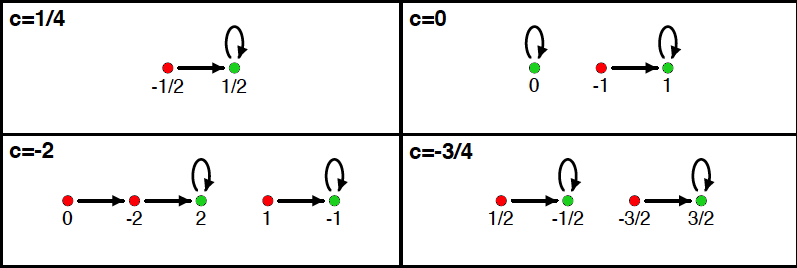
\includegraphics[width=1.0\linewidth]{placeholder}
\end{center}
Diagrams of purely preperiodic points (red) and periodic points (green) of  $f_c(z)=z^2+c$ in $\QQ$.
\end{frame}

\begin{frame}
\begin{center}
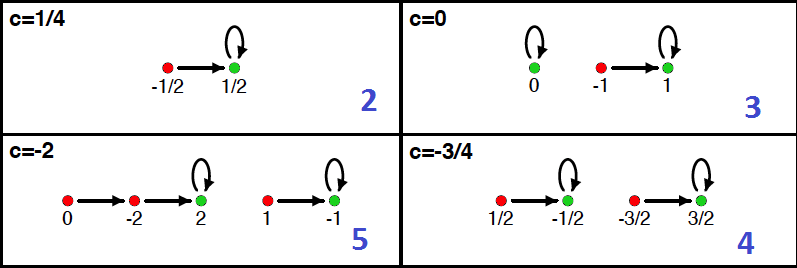
\includegraphics[width=1.0\linewidth]{placeholderNumber}
\end{center}
Diagrams of purely preperiodic points (red) and periodic points (green) of  $f_c(z)=z^2+c$ in $\QQ$.
\end{frame}



\begin{frame}
\begin{center}
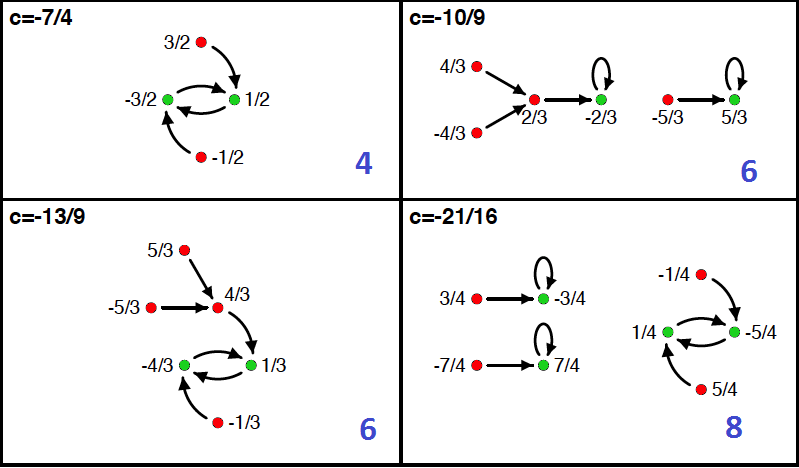
\includegraphics[width=1.0\linewidth]{placeholder2Number}
\end{center}
Diagrams of purely preperiodic points (red) and periodic points (green) of  $f_c(z)=z^2+c$ in $\QQ$.
\end{frame}

\begin{frame}

\textbf{Conjecture:}

Let $f$ be a quadratic polynomial of the form $f_c(z)=z^2+c$ with $c\in\QQ$. Then
$$|PrePer(f_c,\QQ)| \leq 8 $$

\end{frame}

\begin{frame}
\sout{\textbf{Conjecture:}}  \textbf{Question:}

Let $f$ be a quadratic polynomial of the form $f_c(z)=z^2+c$ with $c\in\QQ$. Then
$$|PrePer(f_c,\QQ)| \leq 8 $$

\jump
\Huge{\textbf{USE SAGE}}
\end{frame}


\begin{frame}
\frametitle{Poonen's Conjecture}
\begin{conjecture}[Poonen's Conjecture
  1998]
Let $f:\QQ \to \QQ$ be a quadratic polynomial with coefficients in $\QQ$. Then 
$$|\text{PrePer}(\phi,\QQ)| \leq 8.$$
\end{conjecture}

\vspace{10mm}

If $f = x^2 + d$ then B. Hutz and P. Ingram have shown that Poonen's
conjecture holds when the numerator and denominator of $d$ don't exceed
$10^8$.

\end{frame}


\begin{frame}
PART II:
\begin{itemize}
\item Extra hypothesis: Good/Bad Reduction.
\item Results
\end{itemize}
\end{frame}

\begin{frame}
\frametitle{Good/Bad Reduction}
Let $\pid$ be a prime number in $\ZZ$ and $f(x)=\frac{a_d}{b_d}x^d+\ldots+\frac{a_1}{b_1}x+\frac{a_0}{b_0}$ be a polynomial with coefficients in $\QQ$.

\pause \vspace{8mm}
\begin{itemize}
\item We say that $f$ has \textbf{good reduction} at $\pid$ if $\pid \nmid a_d$ and $\pid \nmid b_d$.
\pause \vspace{5mm}
\item Otherwise, we say that $f$ has \textbf{bad reduction} at $\pid$.
\end{itemize}
\jump
\begin{mydef}
Let $S$ be a finite set of primes of $\ZZ$ and $f$ a polynomial of degree $d$ with coefficients in $\QQ$. We say that $f$ has \textbf{good reduction outside } $S$ if $f$ has good reduction at $\pid$ for every $\pid\notin S$.
\end{mydef}
\end{frame}

\begin{frame}
\frametitle{Example}
\begin{enumerate}
\item Consider $f(x)=15x^3+5x-4$.\\
Can you find the primes of bad reduction?\\ \pause \textbf{Yes}, $3$ and $5$ are primes of bad reduction for $f$.
\vspace{3mm}

If we set $S=\{3,5\}$ then $f$ has good reduction outside $S$.

\pause \vspace{5mm}
\item Consider $f(x)=x^7+2x-2$.\\
Can you find the primes of bad reduction?\\ \pause \textbf{No}. 

If we set $S=\emptyset$ then $f$ has good reduction outside $S$.
\end{enumerate}
\pause \vspace{5mm}

If we allow the number of primes of bad reduction as a parameter, much more is known for the cardinality of the set of preperiodic points. 
\end{frame}

\begin{frame}
\frametitle{Bound on the set of preperiodic point} 
\begin{mythm}


Let $f : \QQ\to\QQ$ be a polynomial of degree $d\geq{2}$ with coefficients in $\QQ$. 
Suppose $f$ has good reduction outside a finite set of primes $S$ and denote $s=|S|$. Then \pause
\begin{itemize}
%d^{ \max\left\{(2^{16s-8}+3)\left[12s\log(5s)\right]^{D}, \left[12(s+2)\log(5s+5)\right]^{4D}\right\}}

\item $|PrePer(f,\QQ)|\leq  d^{2^{16s}\left(s\log(s)\right)}$
 \\ J.K.\ Canci and L.\ Paladino (2015).\jump
\item $|PrePer(f,\QQ)|\leq 5\left(2^{16sd^3}\right)+3$
 \\ S.\ Troncoso (2017).\jump
\item $|PrePer(f,\QQ)|\leq \alpha d^2+\beta d+\gamma$ \\  where $\alpha$, $\beta$ and $\gamma$ are roughly $2^{78s}$.
\\ J.K.\ Canci, S.\ Troncoso and S.\ Vishkautsan (submitted).

\end{itemize}
\end{mythm}
\end{frame}


\begin{frame}
\frametitle{Bounds for Preperiodic points}

The previous theorem use some important results like:\pause
\jump
\begin{itemize}
\item Riemann-Hurwitz formula
\pause
\item  Baker's Theorem on existence of periodic points
\pause
\item Kisaka's analysis on Baker's Theorem
\pause
\item Logarithmic $p$-adic chordal distance.
\pause
\item Study the distance between periodic and purely preperiodic points.
\pause
\item Number of solution of the $S$-unit equation.
\end{itemize}
\end{frame}

\begin{frame}
\frametitle{More general setting}
$$\QQ\pause\Longrightarrow \PP^1(\QQ)=\QQ \cup \{\infty\}\pause\Longrightarrow \PP^1(K) $$
where $K$ is a number field \textit{i.e} a finite field extension of $\QQ$.
\pause \vspace{3mm}

\begin{center}
$$f(x)=a_dx^d\ldots+a_1x+a_0 \mbox{ a polynomial with coefficients in } \QQ.$$
$$\pause\Downarrow$$
$$\phi(x)=\frac{p(x)}{q(x)} \mbox{ where $f$ and $g$ are polynomials with coefficients in } \QQ.$$
$$\pause\Downarrow$$
$$\phi(x)=\frac{p(x)}{q(x)} \mbox{ where $f$ and $g$ are polynomials with coefficients in } K.$$
\end{center}
\end{frame}



\begin{frame}
PART III:
\begin{itemize}
\item Current Research
\item Projects
\end{itemize}
\end{frame}

\begin{frame}
\frametitle{Current project}
\Huge{Arithmetic dynamics in higher dimension}
\end{frame}

\begin{frame}
\frametitle{Notation of preperiodic hypersurfaces}
Let $\phi$ be a function (polynomial in several variables) and $H$ an irreducible hypersurface.
\\\quad\\
\pause

\textbf{Periodic hypersurface}: $\phi^n(H)=H$ for some $n\geq{1}$.
\vspace{2mm}
\\\quad\\

\textbf{Preperiodic hypersurface}: $\exists m\geq{0}$ such that $\phi^m(H)$

The set of preperiodic hypersurface is denoted by $HPrePer(\phi,\QQ)$.

The set of preperiodic hypersurface of degree $e$ is denoted by $HPrePer(\phi,\QQ,e)$.
\end{frame}


\begin{frame}
\frametitle{Question:}
\begin{itemize}
\item Is the set $HPrePer(\phi,\QQ)$ finite? 
\end{itemize}
\pause \textbf{No}. 
\vspace{6mm}\pause

\begin{itemize}
\item Is the set $HPrePer(\phi,\QQ,e)$ finite? 
\end{itemize}
\pause \textbf{Yes}. 
\vspace{6mm}\pause



\begin{mythm}[B. Hutz 2016]
Let $\phi$ be a function. Then there are only finitely many preperiodic hypersurfaces of degree $e$.
\end{mythm}
\end{frame}

\begin{frame}
\frametitle{Project 1: Data base of preperiodic hypersurfaces}
\begin{itemize}
\item Use Sage to provide examples of preperiodic hypersurfaces.
\jump
\item The goal is to state ``Uniform Boundedness Conjecture"  and provide evidence for such a conjecture. 
\end{itemize}
 
\end{frame}


\begin{frame}
\frametitle{Project 2: $S$-unit equations and applications}
Let $S$ be a finite set of primes of $\ZZ$ and $\ZZ_S^{*}$ be the group of $S$-units \\ \textit{i.e.} $\ZZ_S^{*}$ is the set of fraction of the form $\displaystyle\frac{a}{b}$ where $a$ and $b$ are not divisible by primes not in $S$.\pause

\begin{itemize}

\item A linear relation of the form $$u+v=1$$  where  $(u,v) \in \left(\ZZ_S^*\right)^2$ is called a $S$-unit equation. \pause
\item Beukers and Schlickewei give an explicit bound  for the number of solution of a $S$-unit equation.\pause
\item An interesting project will be to understand application in mathematics of Beukers and Schlickewei's result.
\end{itemize}
\end{frame}







\begin{frame}
\Huge{THANK YOU}
\end{frame}


\end{document}
